\begin{figure}
    \centering
    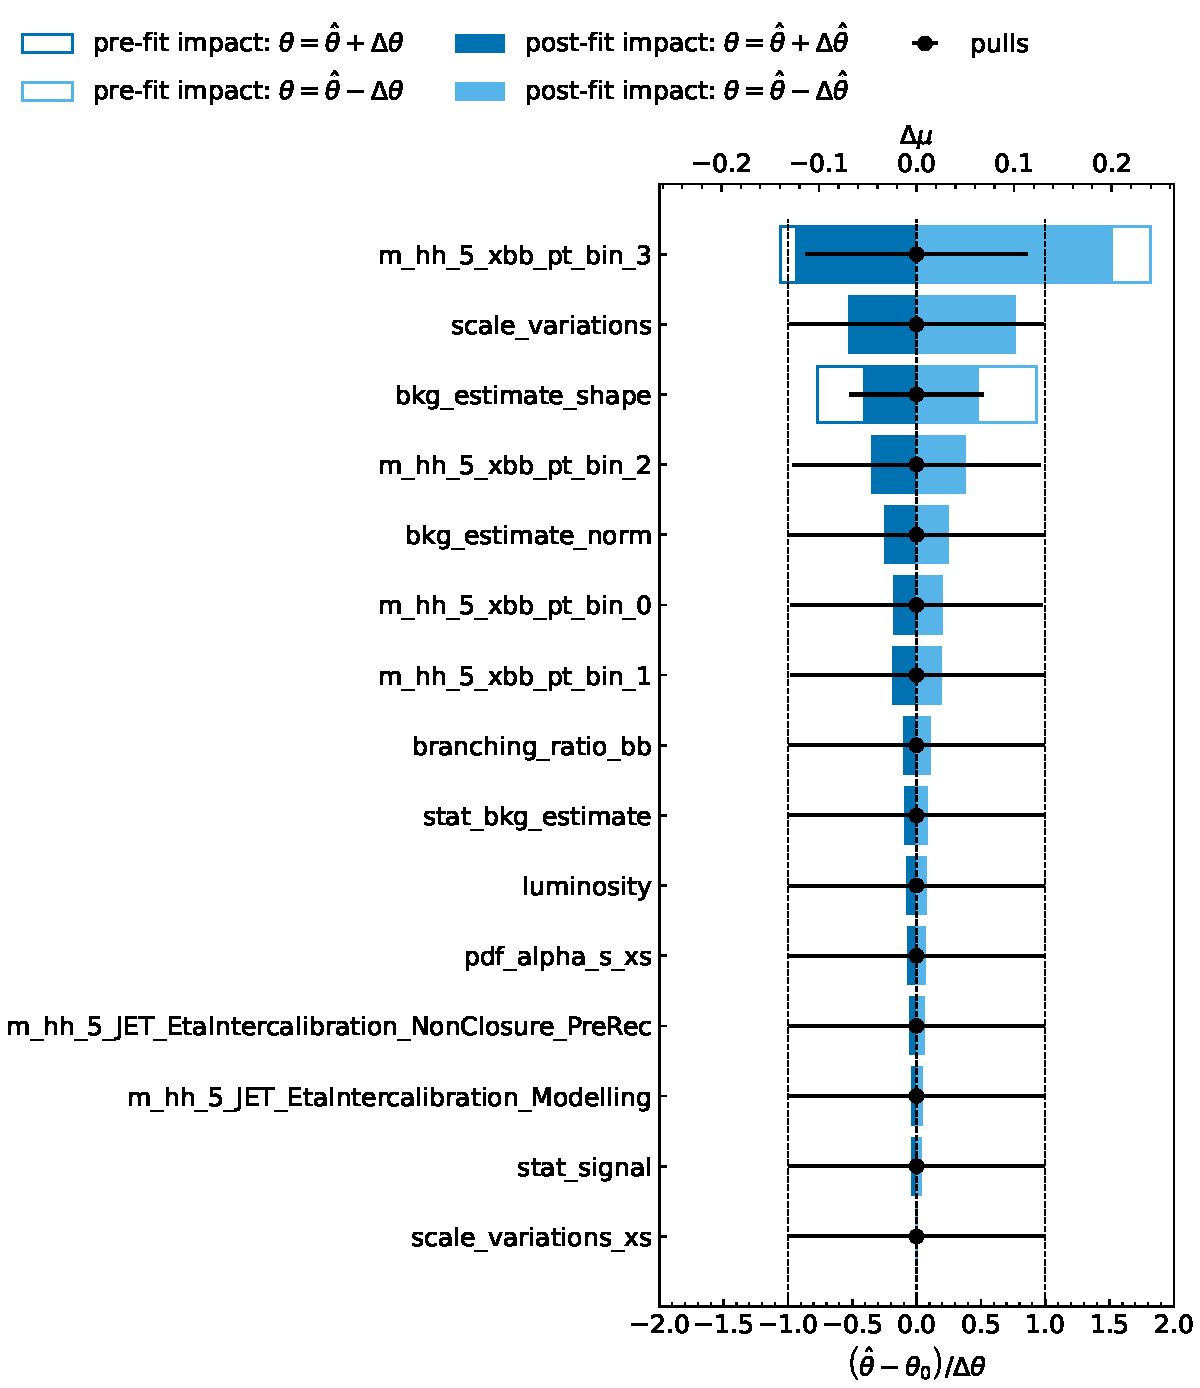
\includegraphics[width=0.22\textwidth]{neos_results/m_hh_5_full_sys_ranking.pdf}
    \caption[]{Ranking of nuisance parameters ordered by their post-fit impact on the signal strength, $\Delta\mu$, displayed on the upper axis for the invariant Higgs Pair mass \mhh{}. The black dots represent the pulls using the lower axis. A detailed explanation of this plot can be found in figure \ref{fig:m_hh_neos_unc_ranking}.}
    \label{fig:m_hh_full_sys_ranking}
\end{figure}
\begin{figure}
    \centering
    \includegraphics[width=0.22\textwidth]{neos_results/tomatos_bce_5_1000_l1cvv0cv1/figures/ranking.pdf}
    \caption[]{Ranking of nuisance parameters ordered by their post-fit impact on the signal strength, $\Delta\mu$, displayed on the upper axis for the \ac{bce}-trained \ac{nn}. The black dots represent the pulls using the lower axis. A detailed explanation of this plot can be found in figure \ref{fig:m_hh_neos_unc_ranking}.}
    \label{fig:bce_full_sys_ranking}
\end{figure}
\begin{figure}
    \centering
    \includegraphics[width=0.22\textwidth]{neos_results/tomatos_cls_5_2500_slope_50_l1cvv0cv1/figures/ranking.pdf}
    \caption[]{Ranking of nuisance parameters ordered by their post-fit impact on the signal strength, $\Delta\mu$, displayed on the upper axis for \ac{neos}. The black dots represent the pulls using the lower axis. A detailed explanation of this plot can be found in figure \ref{fig:m_hh_neos_unc_ranking}.}
    \label{fig:neos_full_sys_ranking}
\end{figure}